\chapter{Fourier Transform Relationship Between Current and Radiation Pattern}
In the previous section, we studied the characteristics of linear dipole/monopole antennas, by modelling them as a collection of Hertz dipoles. 

The current distributions on these dipoles, we saw were sinusoidal. Now, it is worthwhile to ask a question -\textquotedblleft what is the general relationship between the current distribution and the radiation pattern of an antenna?\textquotedblright

If we can establish a general relationship between the current distribution and the radiation pattern, not only will we be able to easily visualize the radiation pattern of different types of antennas, but we will also be able to predict the current distribution for a given radiation pattern. In other words, we will be able to design a current distribution to realize a required radiation pattern.
\begin{figure}[h]
\centering
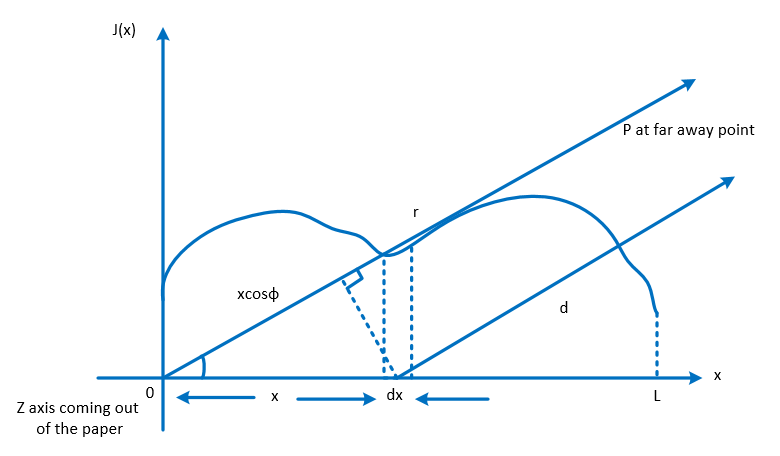
\includegraphics[height=5cm]{./graphics/image53_6}
\caption{Continuous current distribution}
\label{fig:fig6}
\end{figure}

Let us assume a continuous current distribution with linear current density $J(x)$ along $x$ direction as shown in Fig 51.1. The current distribution in general is complex i.e it has a magnitude and a phase.
\begin{equation}
J(x) =
\begin{cases}
|J(x)| e^{j\delta (x)} \ \ \ \ & 0\le x \le L \\
0  & otherwise
\end{cases}
\end{equation}
In practice, these types of current distributions are induces along metal sheets, dielectric sheets, metal wires, apertures etc when they are placed  in an electromagnetic field. Alternatively, we may consider closely spaced antenna elements to appear almost like a continuous current sheet. For example the distribution in Fig \ref{eqn7} can be due to large number of hertz dipoles of length \textquoteleft l\textquoteright oriented perpendicular to the plane of the paper and placed along the $x$ -axis. Then the Hertz dipole can be excited with appropriate currents to mimic the current density J(x) along the $x$ axis.

Let us now consider a small current element of width $dx$ located a distance $x$ from the origin. Since, the direction of the current flow in perpendicular to the plane of the paper, the current element $dx$ has isotropic radiation pattern in the plane of the paper. Now let consider an observation  point P, at a far away distance r in the direction $\phi$ from the $x$ axis, and also a distance d from the current element $dx$ such that

$$d= r- x\cos\phi$$

The  current in the current element is $J(x)dx$ and so the radiation field due to the current element can be written from $$ E_\theta = \dfrac{j\eta\beta Idl\sin\theta e^{-j\beta r}}{4\pi r} $$
as

\begin{equation}
dE = \dfrac{j\eta J(x) Idx\beta\sin\theta e^{-j\beta d}}{4\pi d}
\label{eqn27}
\end{equation} 

for the far away point r $\gg$ x so distance d at the denominator can  be approximated to r but however d in the $ e^{j\beta d}$ can not be approximated because at r $\gg$ x, the amplitude of E does not vary significantly with x, however the phase (which is  $\beta x\cos\theta$ ) has large variation if x is comparable to $\lambda$  so equation \ref{eqn27} is written as

$$ dE = \dfrac{j\eta\beta l\sin\theta e^{-j\beta (r-x\cos\phi)}}{4\pi r}.J(x)dx $$
The  total radiation field at P due to the whole current distribution can be obtained by integrating from  $x = 0$ to $x = L$ as 
$$ E(\phi) = \int_{0}^{L}\dfrac{j\eta\beta l\sin\theta e^{-j\beta r}}{4\pi r}. J(x) e^{j\beta x\cos\phi}dx $$  

\begin{equation}
= \dfrac{j\eta\beta l\sin\theta e^{-j\beta r}}{4\pi r}\int_{0}^{L} J(x) e^{j\beta x \cos\phi}dx
\label{eqn28}
\end{equation} 

For a given distance r, the quantity outside the  integral sign is constant ie let $$ \dfrac{j\eta\beta l\sin\theta e^{-j\beta r}}{4\pi r} = k $$
Note also that $\sin\theta$ is a constant because in our analysis we are considering a constant $\theta$ plane for the current distribution.
Also since J(x) is zero for $x < 0$ and $x >L$, even if we change the limits of integration from $ -\infty\to +\infty$ In equation \ref{eqn28}  value of integral does not change. Therefore, we rewrite as 

\begin{align*}
E(\phi) &= k\int_{-\infty}^{+\infty}J(x) e^{j\beta x \cos\phi}dx \\
&= k\int_{-\infty}^{+\infty}J(x) e^{j(\frac{2\pi}{\lambda}) x \cos\phi}dx\\
\end{align*}
\begin{equation}
=k\int_{-\infty}^{+\infty}J(x) e^{j2\pi(x/\lambda)  \cos\phi}dx
\label{eqn29}
\end{equation}
If we define $\frac{x}{\lambda} \equiv x'$ as the normalized distance and $\cos\theta = p$ 
the direction cosine, we can write equation \ref{eqn29} as 
$$E(\phi) = k\int_{-\infty}^{+\infty}J(x') e^{j2\pi x' p }dx$$
$$ x' = \frac{x}{\lambda}; \ \ \ dx' = \frac{dx}{\lambda}$$
given $dx = \lambda dx'$ we now have

\begin{equation}
E(p) = k\lambda\int_{-\infty}^{+\infty}J(x') e^{j2\pi x' p}dx'
\label{eqn30}	
\end{equation}

This expression is the fourier transform where  the integral is the fourier integral and it relates the spatial current distribution J(x) and the radiation field distribution E(p). Note that the fourier pair is not spatial length $x$ and angle  $\phi$ but is the normalized distance  ($x/\lambda$) and the direction cosine $ p \equiv \cos\phi$ because the radiation pattern is now a function of the direction cosine p and the current distribution is a function of the normalized distance $x'$.

Since the radiation pattern is always normalized with respect to its maximum, the constant $k\lambda$ does not play any role in computation of the radiation pattern. It should be noted that the radiation pattern is a function of the direction cosine, p and every current distribution have the angle $\phi$ which varies from $0\to\pi$ and therefore p will vary from $-\infty\to +\infty$, the only portion of the fourier transform that is useful lies in the range of p given as $-1 \ to\ 1$. This range is called the visible range of p. This is illustrated in fig \ref{fig:8}
\begin{figure}[h]
\centering
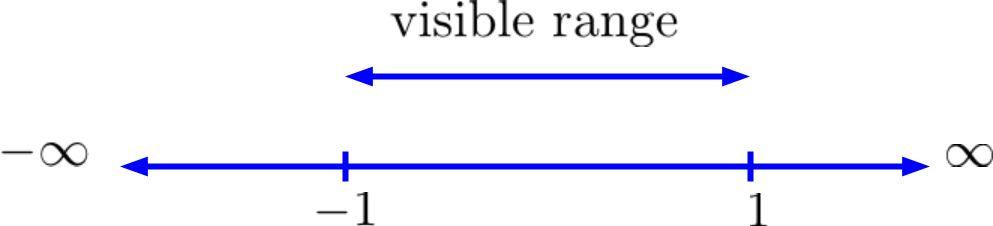
\includegraphics[width=1\linewidth]{./graphics/n8}
\caption{Identification of visible region on linear plot}
\label{fig:8}
\end{figure}

which shows the visible region of the radiation pattern on a linear plot from $-\infty\to +\infty$. Therefore the radiation pattern that lies in this range describes the pattern for the current distribution. So with the fourier transform for a given current distribution we get a unique radiation pattern, however , if we have a radiation pattern we can not get a unique current distribution for instance, if we keep the radiation pattern within the visible region the same and vary the radiation pattern outside the visible region (invisible region) we will get a large number of possible current distributions for the same radiation pattern in the visible region. However it is not possible to choose the radiation pattern outside thee visible range because the function E(p) and its derivatives have to be continuous but what is important to note is that there is no uniqueness in finding the current distribution from a given radiation pattern. So the analysis problem of finding the radiation pattern for a given current distribution is straight forward while the synthesis problem of finding the current distribution for  a desired radiation pattern is not that straight forward because there is no uniqueness in the the solution.

Also it is important to note the fourier integral gives the far field radiation pattern due to distribution of current (i.e current as a function of space $x$ or normalized space $x'$ ). If we consider the current sheet in Fig 51.1, it is like we said, a large collection of hertz dipole and a hertz dipole(intrinsic current element ) has a radiation pattern of $\sin\theta$

Therefore, the total radiation pattern of the current sheet then
is $$E(\theta, \varphi) = E(\varphi)\sin\theta$$
Where $E(\varphi)$ is the radiation pattern for the current distribution which is gotten from the fourier transform, and $\sin\theta$ is the radiation pattern of the intrinsic current element (which are the Hertz dipole).

The theory of fourier transform is very well developed in signal analysis. Therefore, it becomes convenient to visualize the various antennas characteristics through properties and theorems of fourier transform. In the following section we will obtain radiation patterns of an antenna with various current distributions using fourier transform.

\section{Radiation Pattern of a Uniform Current Distribution}
Let's obtain the radiation pattern for a uniform current distribution. Without losing generality, let us the current density be unity over a normalized length $L$ as shown in Fig. \ref{fig9}. Let also assume that there is no phase variation in the current density, $J(x')$.
\begin{figure}[h]
\centering
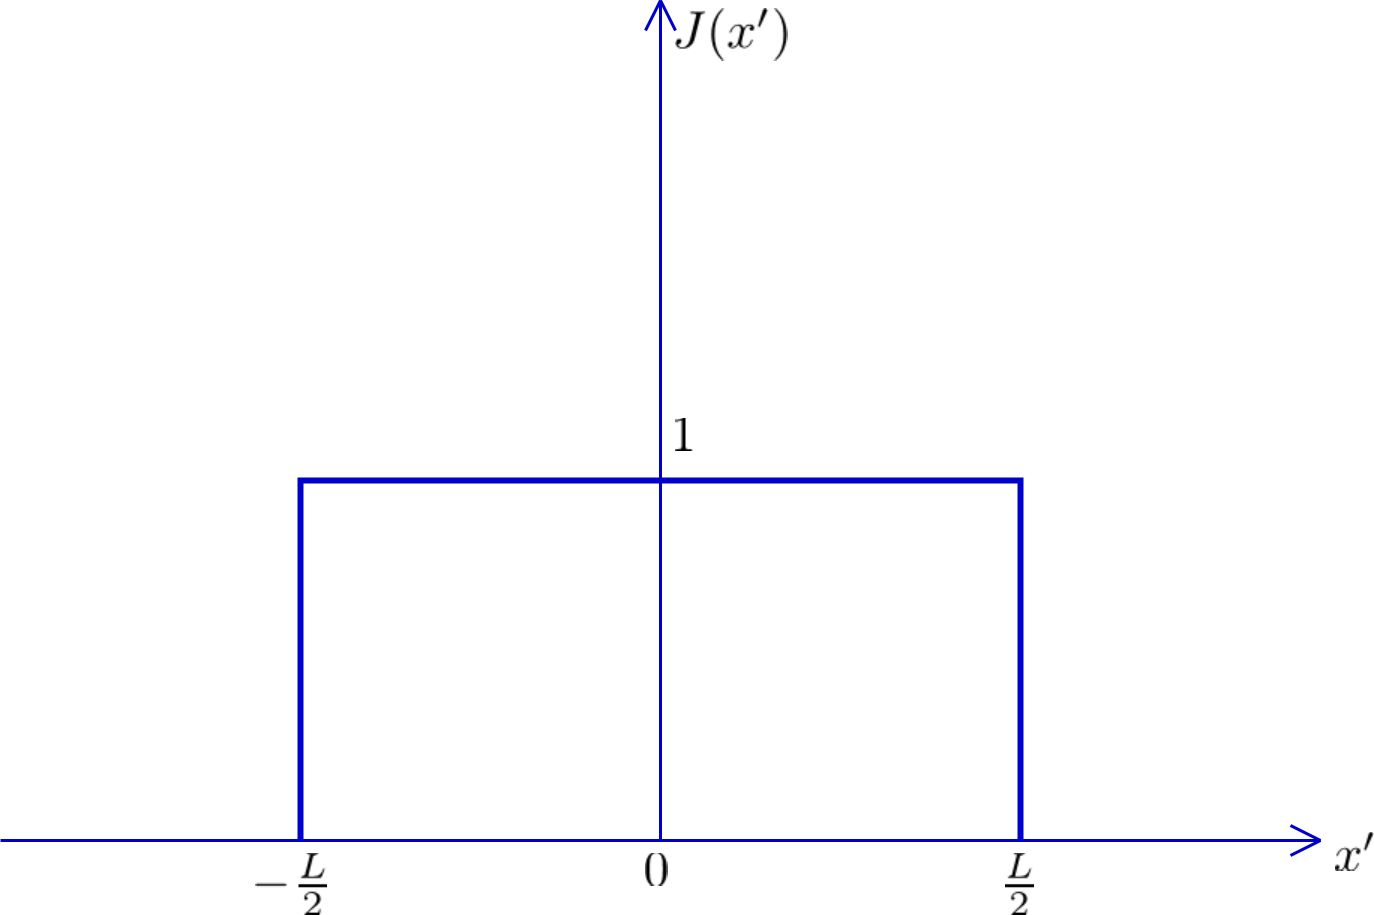
\includegraphics[width=1\linewidth]{./graphics/n9}
\caption{Uniform current Distribution}
\label{fig9}
\end{figure}

We can write the equation of the current distribution in fig 9 as
\begin{equation*}
J(x) =
\begin{cases}
1 \ \ \ \ & \frac{-L}{2}\le x' \le \frac{L}{2} \\
0  & otherwise
\end{cases}
\end{equation*}
Such that the radiation pattern is given by 
\begin{align*}
E(p) &= K_0\int_{\dfrac{-L}{2}}^{\dfrac{L}{2}} 1.e^{j2\pi x'p }dx' \; \; \; \;\text{where}\; \;  K_0 = K\lambda\\ %Resolve issue of Double superscript%
&= K_0\bigg[\dfrac{e^{j2\pi x'p}}{j2\pi p}\bigg]_{\frac{-L}{2}}^{ \frac{L}{2}}\\	  
&= K_0 \bigg\{\dfrac{ e{^j\pi Lp}- e^{-j\pi Lp}}{j2\pi p}\bigg\}\\
%Resolve the error here
& = \dfrac{K_0}{\pi p}\bigg\{\dfrac{ e^{j\pi Lp} -  e^{-j\pi Lp}}{j2}\bigg\} = \dfrac{K_0}{\pi p}\sin(\pi Lp)
\end{align*}
$$E(p) = K_0 \dfrac{\sin (\pi Lp)}{\pi p}$$\\
The maximum value of $E(p)$ will be $K_0L$ and will correspond to $ p = 0$, such that the limit at $p = 0$ is 1. i.e $\lim\limits_{p\rightarrow0} \dfrac{\sin(\pi Lp)}{\pi Lp} = 1$.\\
Normalizing the $E(p)$ with respect to the maximum value, we get the radiation pattern as

\begin{equation}
\dfrac{E(p)}{K_0 L} = \dfrac{\sin(\pi pL)}{\pi pL} = \text{sinc}(pL)
\end{equation}
\\
The uniform current distribution is a sinc function radiation pattern. However, remember, that $p$ is the direction cosine and hence $p$ lies between -1 and +1, whereas when we take fourier transform of $J(x')$ we get $E(p)$ for all values of $p$. Therefore, only the portion of $E(p)$ corresponding to $-1 < p < +1$ gives the visible range of $p$. The function maximum at $p = 0$ i.e $\varphi = \dfrac{\pi}{2}$ represents the main beam.

\begin{figure}[h]
\centering
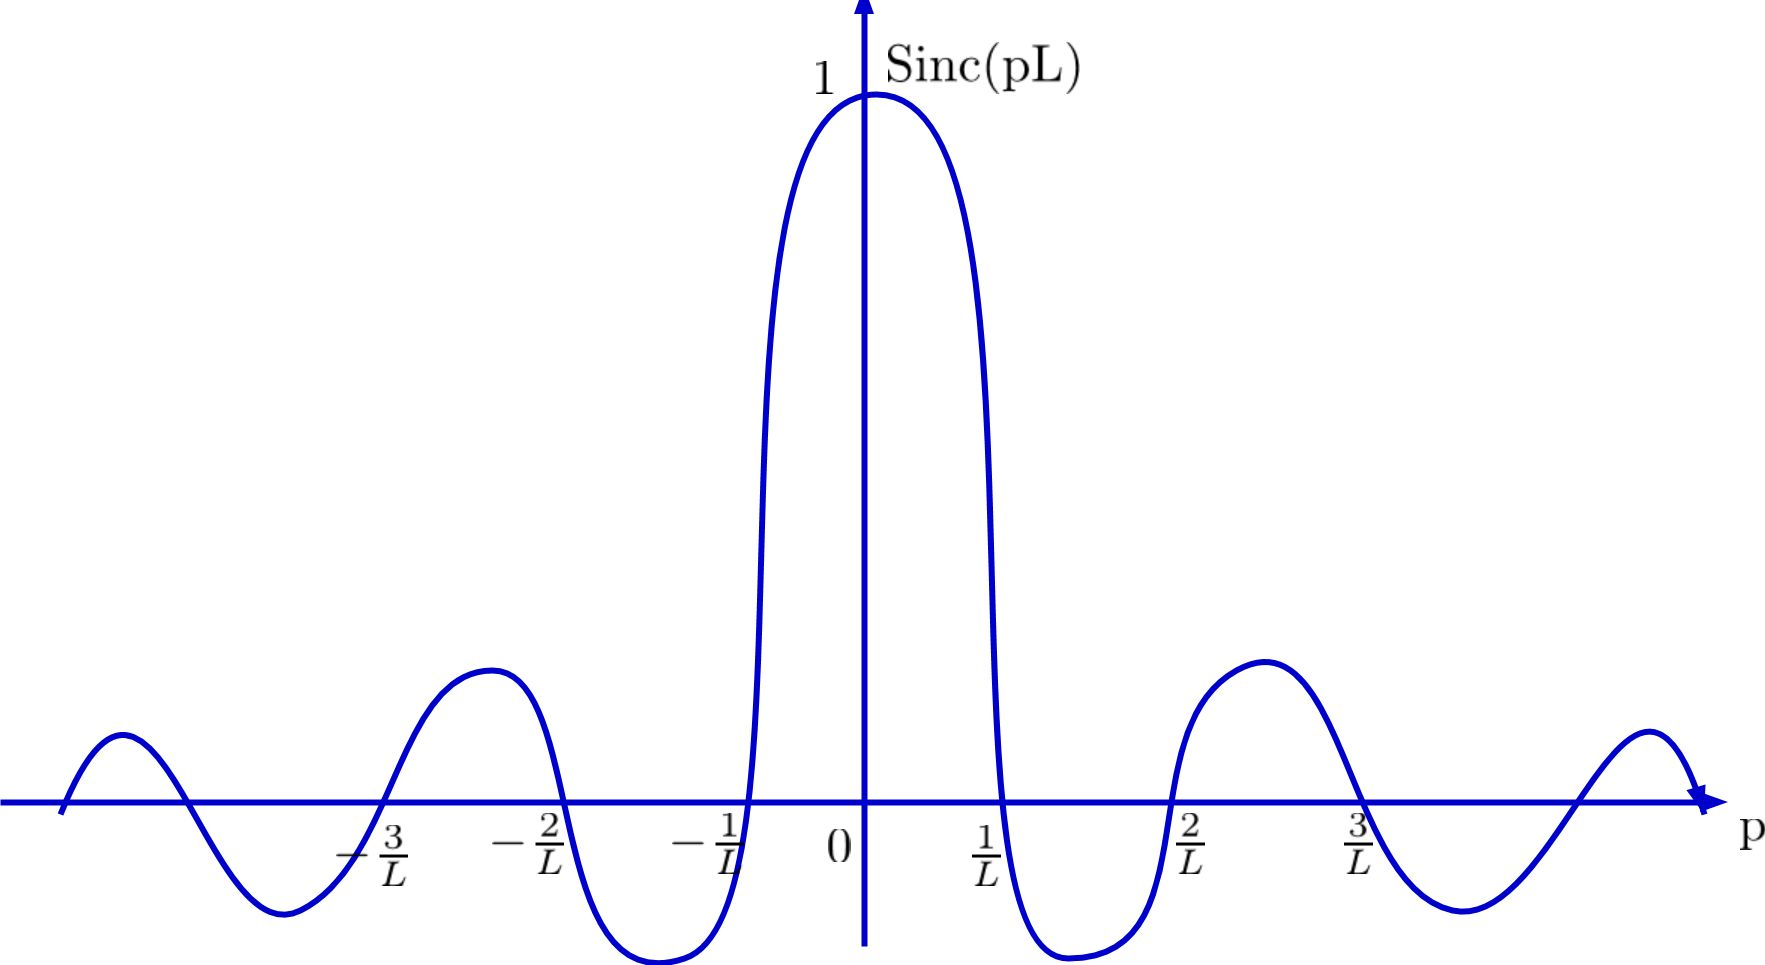
\includegraphics[width=1\linewidth]{./graphics/n10}
\caption{sinc(pL) for visible range of p}
\label{fig10}
\end{figure}

%Fig 10. Sinc(pL) for visible range of p%
The nulls of a sinc function would correspond to when $\pi pL$ is a multiple of $\pi \; \; \text{i.e} \; \; \pi pL = m\pi ; \; \; m = 1, 2, 3, \ldots$ So, $Lp$ will be given an integer so the function has null at $p = \pm\dfrac{1}{L}, \pm\dfrac{2}{L}$ and so on. Also, the local maxima (side lobes) occurs at $p = \pm\dfrac{3}{2L}, \pm\dfrac{5}{2L}$ and so on.

As we can be seen from fig.\ref{fig10}, the nulls and side lobes are equi-spaced along $p$ by a distance of $\dfrac{1}{L}$.

Substitution of $p = \dfrac{3}{2L}, \dfrac{5}{2L}$ etc in equation \ref{eqn31}, we get the amplitudes of the side lobes as $-\dfrac{2}{3\pi}, \dfrac{2}{5\pi}$ etc respectively. That is, the amplitude of the first side lobe is $21\% $ of the peak and the second side lobe is about $13\%$ of the peak. One other important fact to be noted is if we increase the width of the current distribution (such as from $-L$ to $+L$), this is the same as increasing the length of the current sheet and we observe that the width of the main beam reduces\footnote{From fig 10; we observe that the width of the beam is $\dfrac{2}{L}$ and therefore the beam width varies as $\dfrac{1}{L}$} (i.e the beam width between first nulls decreases) and the beam becomes narrower. Therefore, as the size (aperture) of the antenna increases, the antenna becomes more directive, and also the more nulls we get\footnote{Also we observe there are approximately $2L$ nulls, so as $L$ increases, the number of null increases.}.

\section{Tilting the Main Beam.}
Let's consider for instance a case when we have to change the direction of the beam, say, by $p_0$, we should notice that $p_\circ$ is the direction cosine and it corresponds to an angle $\phi_\circ$ on the polar plot. So it is equivalent to tilting the beam by $\phi_\circ$ and then we wanted to know how the current distribution would get affected. Therefore we can substitute for $p$ in the fourier transform by $(p - p_\circ)$, such that;
$$E(p - p_\circ) = K_\circ\int_{-\infty}^{\infty} J(x') e^{j2\pi (p - p_\circ)x'} dx'$$
$$= K_\circ\int_{-\infty}^{\infty} J(x') e^{j2\pi px'}  e^{-j2\pi p_\circ x'} dx'$$
Rewriting the expression,
$$= K_\circ\int_{-\infty}^{\infty} [J(x') e^{-j2\pi p_\circ x'}] e^{j2\pi px'} dx'$$
$$ = K_\circ\int_{-\infty}^{\infty} [J(x') e^{j\delta (x')}] e^{j2\pi px'} dx ;\; \; \; \; \; \delta(x') = -2\pi p_\circ x'$$
What it shows us is that the radiation pattern $E(p - p_\circ)$ which is shifted by $p_0$ is the fourier transform of  $J(x')e^j\delta(x')$ and this current distribution has a phase $\delta(x')$ given as $-2\pi p_0x'$ which shows linear variation with $x'$ as shown in fig \ref{fig11}. Hence any linear phase change in the current distribution will rotate the radiation pattern in the $\varphi$ domain or in $p$ domain and it is called the shift property of fourier transform. That is if the function is shifted in one domain, it is equivalent to a phase gradient in the other domain and vice versa.
%Fig 11%
\begin{figure}[h]
\centering
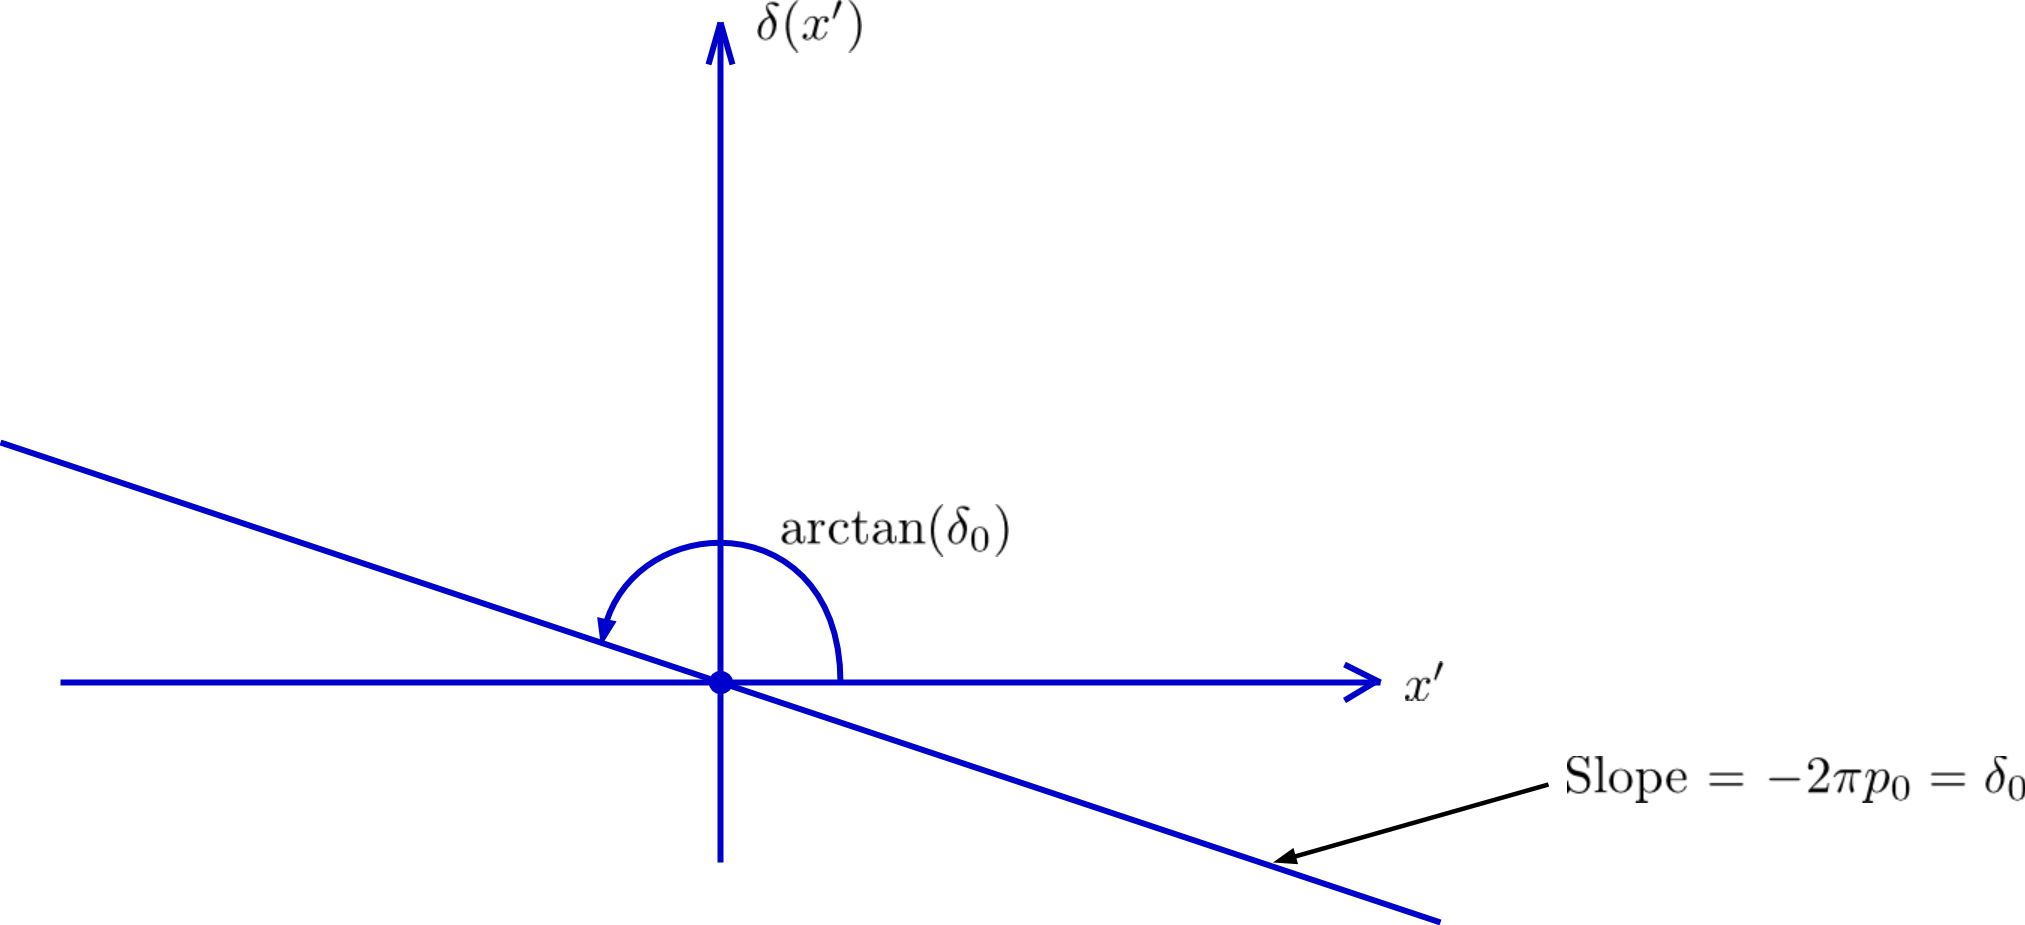
\includegraphics[width=1\linewidth]{./graphics/n11}
\caption{phase variation of current distribution}
\label{fig11}
\end{figure}

So, without mechanical movement of the antenna, the radiation pattern or the beam can scan through space just by introducing a linear phase gradient $\delta_0$ in the current distribution. For a negative phase gradient (which we are considering) the beam tilt towards the right while for a positive phase gradient, the beam tilt towards the left.

For a uniform current distribution we observe the first side lobe level is -21 percent irrespective of the size of the antenna (because it is one of the properties of the sinc function and it is independent of L). So, no matter the value of $L$ the side lobe level is always -21 percent. The side lobes are essentially leakage of power in unwanted direction and it is required that we reduce the side lobes level. The side lobe levels which are ripples in the fourier transform (sinc function) are due to discontinuity in the current distribution in space. Therefore, if we avoid the abrupt change at the ends of the current distribution (i.e for the case we are studying, $\dfrac{-L}{2}$ and $\dfrac{L}{2}$) then the ripple can reduce. This is called tapering of the current distribution. Let's consider fig.\ref{fig12} for different levels of tapering of the current distribution and the resulting radiation pattern.
\begin{figure}[h]
\centering
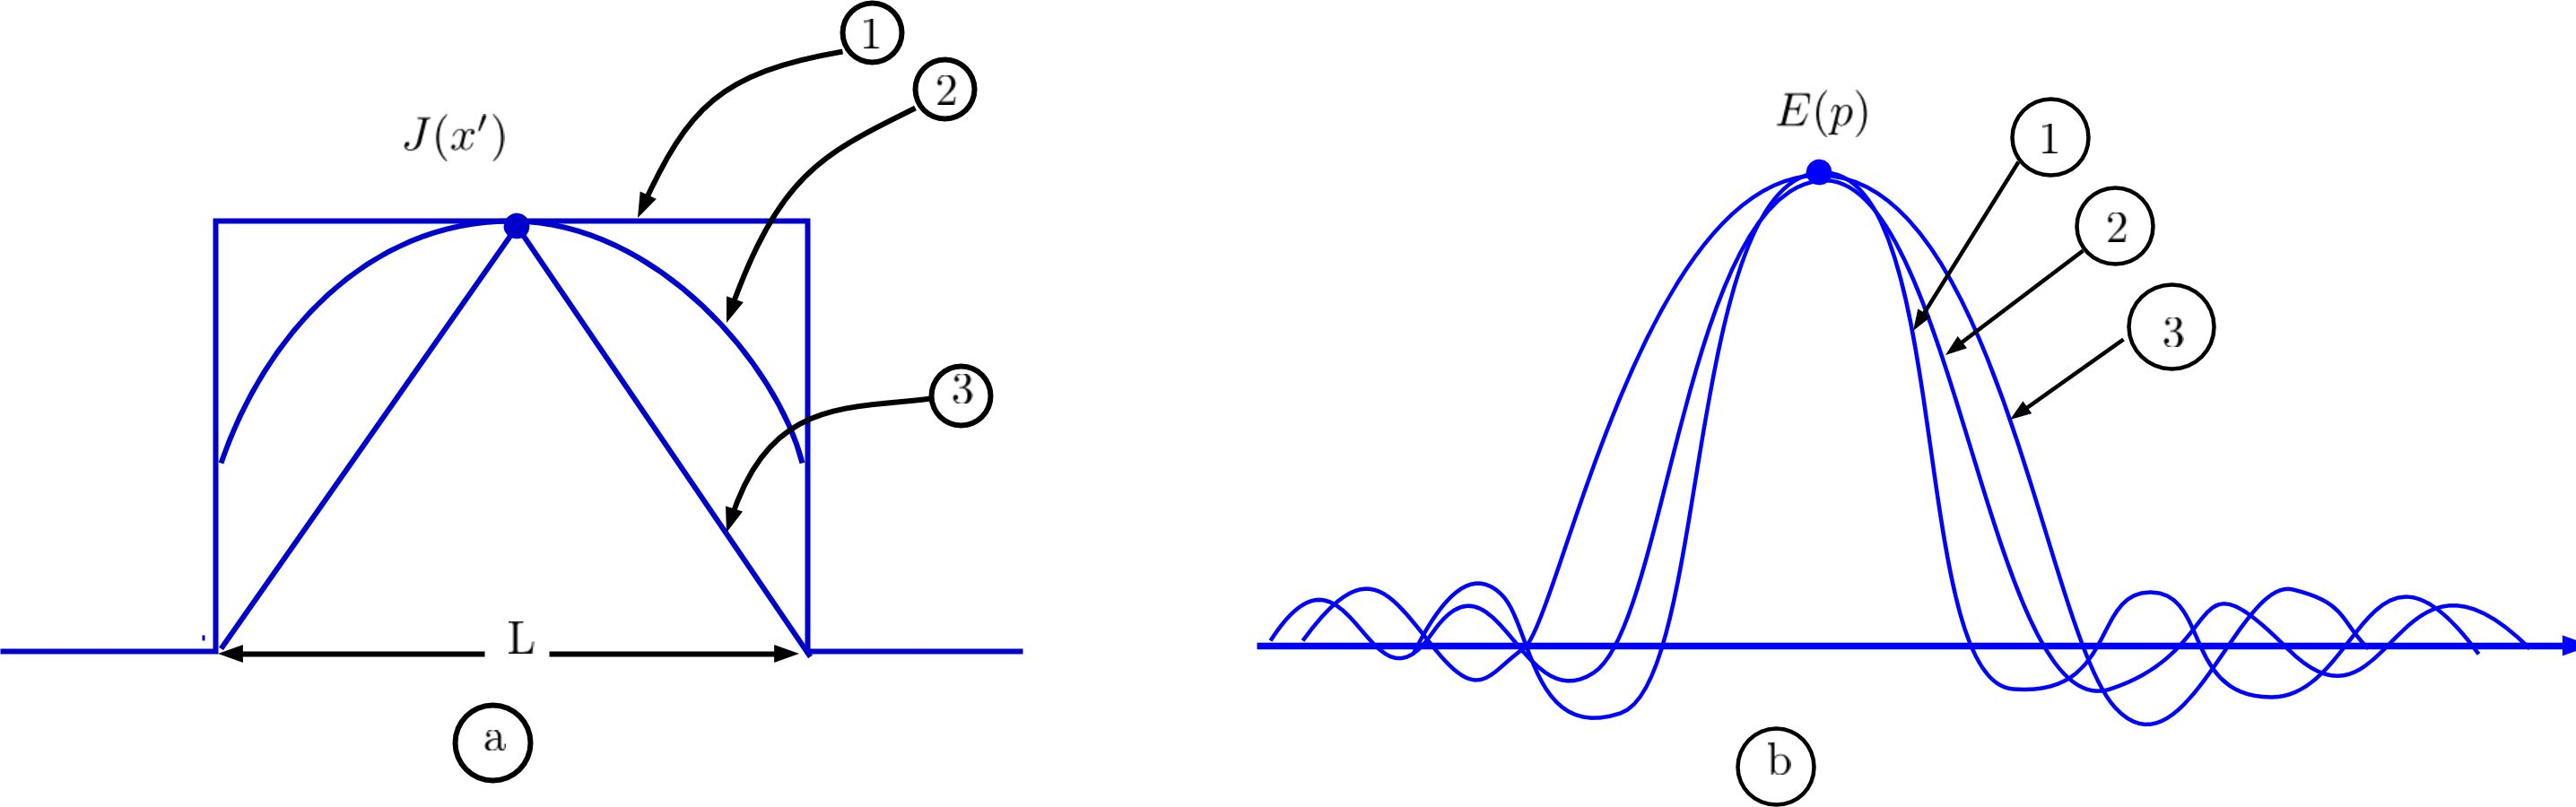
\includegraphics[width=1\linewidth]{./graphics/n12}
\caption{Current distribution and their respective effect on the side lobes}
\label{fig12}
\end{figure}

%Fig.12 : Current distribution and their repective effect on the side lobes.
It can be seen that as the tapering increases, the side lobe levels reduces, however the beam width becomes larger which means the directivity reduces. This is because tapering the current distribution is equivalent to a current distribution of shorter length $l < L$ (it is equivalent to defining 3dB points for the current distribution which reduces the length of the current distribution) hence as the size of the current distribution reduces, the beam width increases. So we observe there is a trade-off between the sidelobe levels and the directivity of the antenna.


The most important property of the fourier transform which is used is the convolution property. For instance if we have 2 functions $f_{1}(x),\ f_2(x)$ and
their fourier transform pair $F_1(p),\ F_2(p)$ respectively, from the convolution theorem the fourier transform of the product of $f_{1}(x)$ and $f_{2}(x)$ is equal to the convolution of the fourier transform of $f_1(x)$ and $f_2(x)$ which is $F_{1}(p)$ * $F_{2}(p)$ and also the convolution of $f_{1}(x)$ and $f_{2}(x)$ is the product of the fourier transform of $f_{1}(x)$ and $f_{2}(x)$ gives as $F_{1}(p)$ $F_{2}(p)$ .This convolution property is used to quickly find the pattern of complex current distribution .


For instance, lets consider a case of a triangular current distribution as shown in \ref{fig:n13} and we would want to find the radiation pattern for this distribution. Then, the current distribution is the convolution of two rectangular current distributions length $\dfrac{L}{2}$ .The two rectangular current distributions are uniform current distributions and we have consider it in the previous section
\begin{figure}[h]
\centering
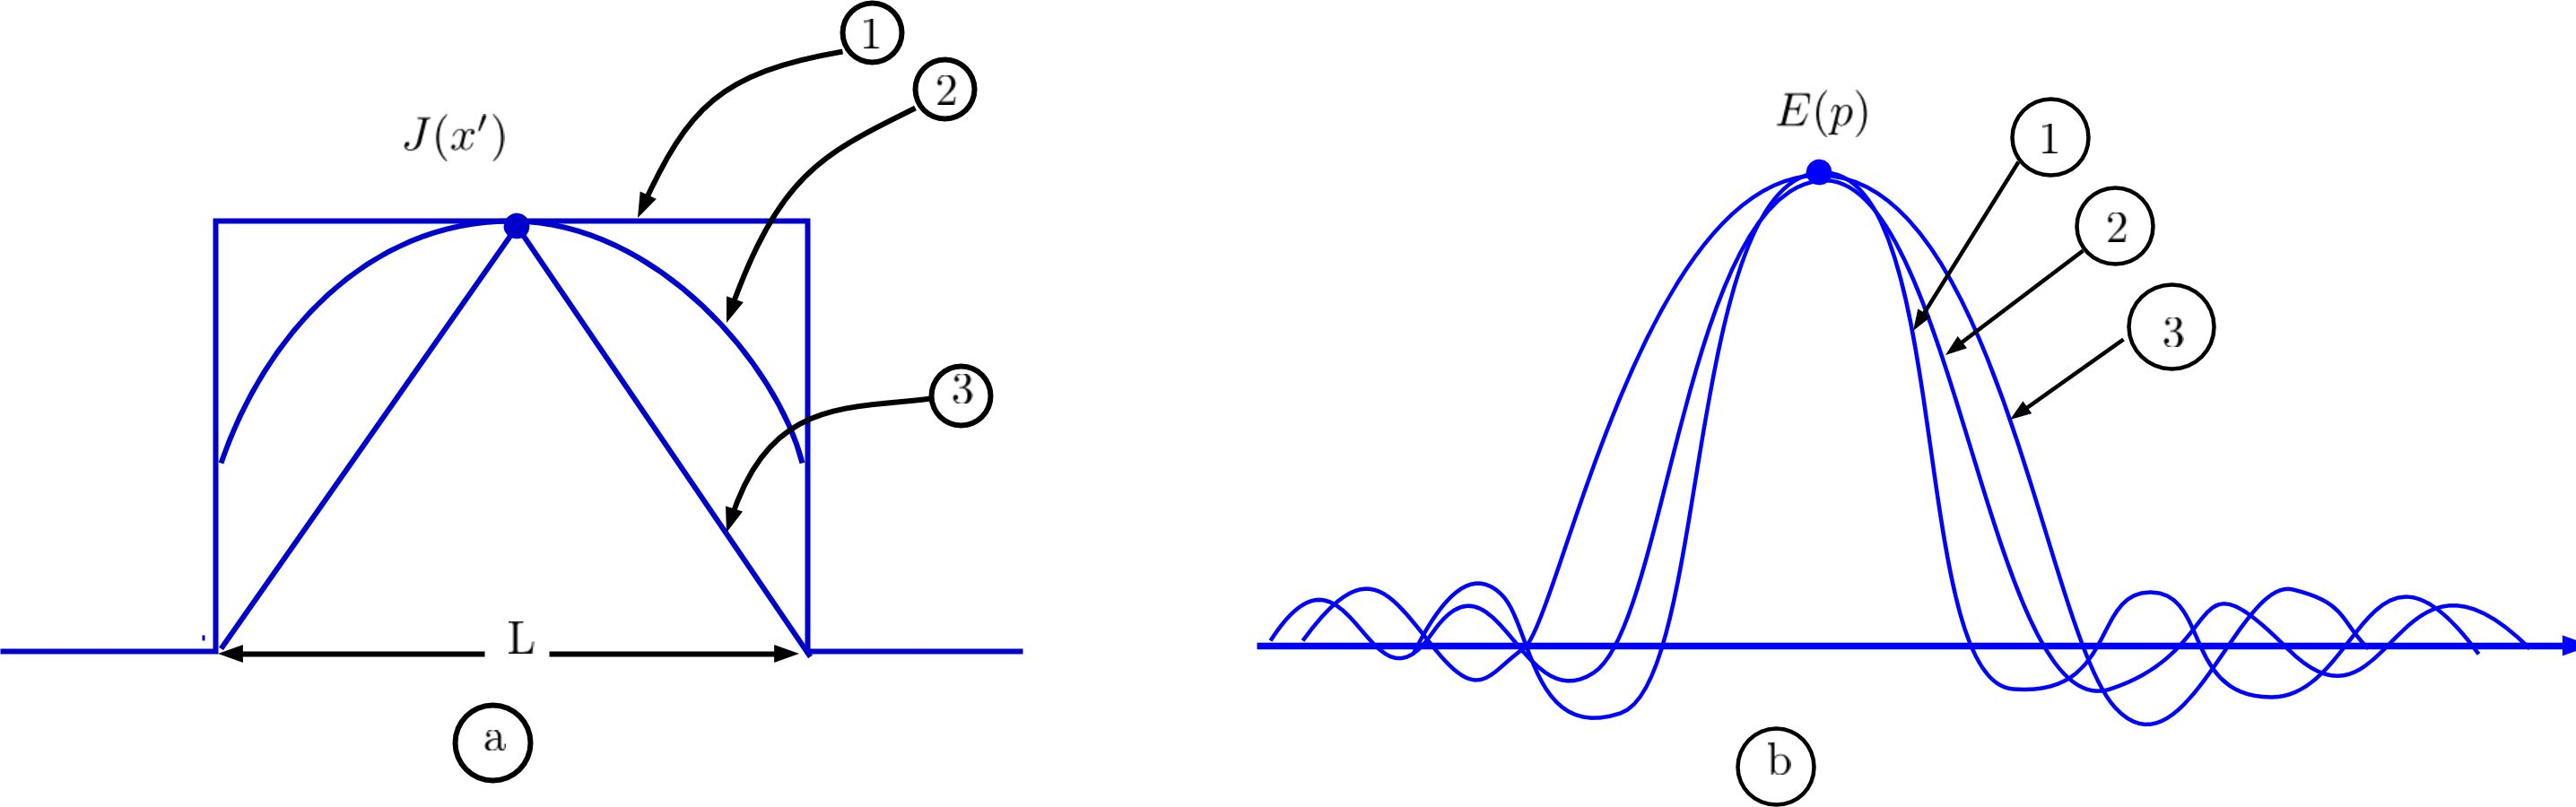
\includegraphics[width=1\linewidth]{./graphics/n12}
\caption{Convolution of two rectangular current distribution of length $\dfrac{L}{2}$ gives a triangular current distribution of length L}
\label{fig:n13}
\end{figure}

Therefore, the fourier transform of the triangular current distribution will be given as

\begin{equation*}
E(p) =  \ E_1(p) E_{2}(p) = J_{1}(x') * J_{2}(x')
\end{equation*}

Recall, for uniform current distribution of length, $\dfrac{L}{2}$, is;

$$
E_{1}(p) = \dfrac{K_{o}L\text{sinc}}{2} \left(\dfrac{\rho L}{2}\right)$$

$$
E_{2}(p) = \dfrac{K_{o}L\text{sinc}}{2} \left(\dfrac{\rho L}{2}\right)$$
where $E_{1}(p)$ is the radiation pattern for rectangular current distribution 1
and $E_2(p)$ is the radiation pattern for rectangular current distribution 2.

Now let's normalize the fourier transform E(p) for both distribution, we have;\\
$\dfrac{2E_1(p)}{K_0L} = sinc(\dfrac{pL}{2})$ and $\dfrac{2E_2}{K_0L} = sinc(\dfrac{pL}{2})$.\\
So the radiation pattern of the triangular current distribution $J(x')$ given as $E_n(p)$ is;
\begin{equation}
E_n(p) = \text{sinc}^2\left(\dfrac{pL}{2}\right)
\end{equation}  
Where $E_n(p) = \dfrac{E(p)}{E_{max}(p)}$.This is the radiation pattern of the triangular current distribution and if we consider the magnitude of the first side lobe, it will reduce to 0.04 because for the uniform distribution the first side lobe level was 0.21 and since the radiation pattern for the triangular current distribution is the square of that of the uniform current distribution, we have that $(0.21)^2$ is approximately 0.04 or 4 per cent. Also, the next sidelobe will have a magnitude of approximately 0.016 and so on. So the triangular distribution will give a side lobe of 4 percent which is like considering a current distribution which has been tapered such that the ends go to zero at $-\dfrac{L}{2}$ and $\dfrac{L}{2}$.

In conclusion, we got a relationship which is the Fourier transform for examining the radiation pattern of an antenna given the current distribution. Now, it can be said that if a given current distribution will give a unique radiation pattern, then controlling the current distribution has a way of controlling the radiation pattern. However, it is not possible to control the current because just as it was explained in the case of the dipole, the current cannot be controlled but the length of the dipole can be controlled and as we vary the length, the terminal impedance varies. So, we have that the current distribution which is related to the radiation pattern is coupled to the terminal impedance. Therefore, we are in search of a mechanism by which the current can be independently controlled without affecting the terminal characteristics and it would be treated in the topic arrays in the next chapter.